\documentclass[12pt]{article}
\usepackage{graphicx}
\usepackage{geometry}
\usepackage{fancyhdr}
\usepackage{titling}
\usepackage{amsmath}
\usepackage{amssymb}
\usepackage{enumitem}
\usepackage{xcolor}
\usepackage{circuitikz}
\usepackage{tikz}
\usepackage{subfigure}

\geometry{a4paper, margin=1in}

\title{\textbf{EE1200 - ELECTRIC CIRCUITS LAB}}
\author{EE24BTECH11012 - Bhavanisankar G S \\ EE24BTECH11019 - Dwarak A}
\date{\today}

\pretitle{%
    \begin{center}
    
\includegraphics[width=0.5\textwidth]{IITH.png}\\
    \vspace{1cm}
    \LARGE
}
\posttitle{\end{center}}

\begin{document}

\maketitle
\thispagestyle{empty}

\newpage

\section{BAND-PASS FILTER USING SALLEN-KEY SECOND-ORDER FILTERS}

\subsection{\textbf{AIM} : } 
\begin{itemize}
	\item To design and implement a band-pass filter using separate Sallen-Key Low Pass Filter ( LPF ) and High Pass Filter ( HPF ) .
	\item To analyze and compare the frequency response of LPF, HPF, and the final bandpass filter.
	\item To plot the magnitude response ( gain vs frequency ) of all the three filters.
\end{itemize}

\subsection{\textbf{APPARATUS REQUIRED} : }
\begin{itemize}
	\item Breadboard
	\item Op-Amps
	\item Four resistors
	\item Four capacitors
	\item Oscilloscope
	\item Digital function generator
	\item DC Power supply
	\item Connecting wires
\end{itemize}

\subsection{\textbf{THEORY} : }
A bandpass filter allows signals within a specific frequency range (\textit{passband}) to pass while attenuating frequencies outside this range. This can be achieved by cascading a high-pass filter (HPF) and low-pass filter (LPF), where:

\begin{itemize}
    \item HPF sets the lower cutoff frequency ($f_{low}$)
    \item LPF sets the upper cutoff frequency ($f_{high}$)
    \item Bandwidth $B = f_{high} - f_{low}$
\end{itemize}
The combined frequency response exhibits:
\begin{itemize}
    \item -20 dB/decade roll-off below $f_{low}$
    \item -20 dB/decade roll-off above $f_{high}$
    \item Flat response between $f_{low}$ and $f_{high}$
\end{itemize}

For first-order filters, the transfer functions are:
\begin{equation}
    H_{HP}(s) = \frac{sRC_{HP}}{1 + sRC_{HP}}
\end{equation}
\begin{equation}
    H_{LP}(s) = \frac{1}{1 + sRC_{LP}}
\end{equation}

The combined bandpass transfer function becomes:
\begin{equation}
    H_{BP}(s) = H_{HP}(s) \cdot H_{LP}(s) = \frac{sRC_{HP}}{(1 + sRC_{HP})(1 + sRC_{LP})}
\end{equation}
The cutoff frequencies are determined by:
\begin{equation}
    f_{low} = \frac{1}{2\pi R_{HP}C_{HP}}
\end{equation}
\begin{equation}
    f_{high} = \frac{1}{2\pi R_{LP}C_{LP}}
\end{equation}
\begin{itemize}
    \item Cascading order affects roll-off slope (-40 dB/decade for second-order)
    \item Component tolerance impacts actual cutoff frequencies
    \item Loading effects between stages may require buffer amplifiers [5][8]
    \item Quality factor $Q = \frac{f_0}{B}$, where $f_0 = \sqrt{f_{low}f_{high}}$
\end{itemize}
The ideal bandpass response can be represented as:
\begin{equation}
    |H(f)| = \begin{cases}
        1 & \text{if } f_{low} \leq f \leq f_{high} \\
        0 & \text{otherwise}
    \end{cases}
\end{equation}

A Sallen-key second order is an active filter topology made using operational amplifiers. It provides a Butterworth, Bessel or Chebyshev response based on component selection. The corresponding transfer function is given by - 
\begin{equation}
	H(s) = \frac{A}{s^2 + \frac{\omega_{c}}{Q}s + \omega_{c}^2}
\end{equation}
\begin{equation}
	\omega_{c} - \text{ Cut-off frequency } \\
	Q - \text{ Quality Factor }
\end{equation}


\subsection{\textbf{CIRCUIT DESIGN} : }
The three types of filters are shown in Figure \ref{fig:lpf}, Figure \ref{fig:hpf} and Figure \ref{fig:bpf}
\begin{figure*}[!htb]
    {\centering 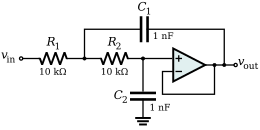
\includegraphics[ width=0.31\textwidth]{LPF.png} \caption{Low Pass Filter} \label{fig:lpf}}
    \vspace{\fill}
    {\centering 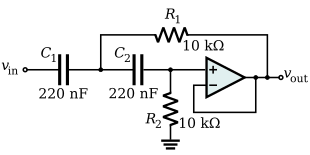
\includegraphics[ width=0.31\textwidth]{HPF.png} \caption{High Pass Filter} \label{fig:hpf}}
    \vspace{\fill}
    {\centering 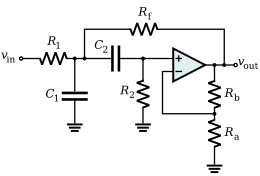
\includegraphics[ width=0.31\textwidth]{BPF.png} \caption{Band Pass Filter} \label{fig:bpf}}\\
\end{figure*}

\subsection{\textbf{PROCEDURE} : }
\begin{itemize}
	\item Connect the HPF circuit as shown in the circuit diagram.
	\item A sine wave input is given using the digital function generator. The input frequency is varied and the output voltage is measured.
	\item The gain value is recorded for different frequencies, and is plotted against frequency ( Bode Plot ).
	\item Repeat the same steps with LPF and Bandpass filters.
\end{itemize}

\subsection{\textbf{OBSERVATION : }}
\begin{itemize}
	\item The frequency response of HPF, LPF and Bandpass filters can be seen in the figures attached.
	\item Experimental cutoff frequency = 
	\item Theoritical cut-off frequency =
	\item Frequency range of Bandpass filter = 
\end{itemize}

\subsection{\textbf{RESULT} : }
\begin{itemize}
	\item Cut-off frequency =
	\item Roll-off slope = 
	\item Phase difference goes from 90 $\degree$ to 0 $\degree$ 
\end{itemize}
\end{document}

